% Created 2017-11-20 Mon 23:41
\documentclass[11pt]{article}
\usepackage[utf8]{inputenc}
\usepackage[T1]{fontenc}
\usepackage{fixltx2e}
\usepackage{graphicx}
\usepackage{longtable}
\usepackage{float}
\usepackage{wrapfig}
\usepackage{rotating}
\usepackage[normalem]{ulem}
\usepackage{amsmath}
\usepackage{textcomp}
\usepackage{marvosym}
\usepackage{wasysym}
\usepackage{amssymb}
\usepackage{hyperref}
\tolerance=1000
\usepackage{minted}
\usepackage{fancyhdr}
\setcounter{secnumdepth}{-1} 
\pagestyle{fancy}
\fancyhead{} 
\rhead{\textit{Michael Laufer}}
\lhead{\textit{Numerical Methods Fall 2017, HW6}}
\small

\author{Michael Laufer}
\date{\today}
\title{HW3 Numerical Methods Fall 2017}
\hypersetup{
  pdfkeywords={},
  pdfsubject={},
  pdfcreator={Emacs 25.3.1 (Org mode 8.2.10)}}
\begin{document}

\maketitle
\section{ADI Iterative Scheme - 4th Order Poisson}
\label{sec-1}
\subsection{Problem}
\label{sec-1-1}
Given the Poisson equation:
\[
\frac{\partial^{2} \phi}{\partial x^{2}} + \frac{\partial^{2} \phi}{\partial y^{2}} = S_{\phi}
\]
Where $S_{\phi}$ is defined as:
\[
S_{\phi} = 2\sinh { 10 (x- \frac{1}{2})] + 40(x-\frac{1}{2}) \cosh [ 10 ( x - \frac{1}{2})^{2} )]+
\]
\[
100 ( x - \frac{1}{2} )^{2} \sinh [10 ( x- \frac{1}{2} ) ] + 2\sinh { 10 (x- \frac{1}{2})] +
\]
\[
40(x-\frac{1}{2}) \cosh [ 10 ( x - \frac{1}{2})^{2} )]+ 100 ( x - \frac{1}{2} )^{2} \sinh [10 ( x- \frac{1}{2} )]+
\]
\[
4( x^{2} + y^{2}) exp(2xy)
\]
Derichlet boundary conditions are given as functions defined on the unit square domain boundary. \\
The system has an analytical solution given by:
\[
\phi \left( x,y \right) = \left( x - \frac{1}{2} \right)^{2} \sinh \left[10 \left( x - \frac{1}{2} \right) \right] + \left( y - \frac{1}{2} \right)^{2} \sinh \left[10 \left( y - \frac{1}{2} \right) \right] + exp(2xy) 
\]

\subsection{Solution Methodology}
\label{sec-1-2}
The problem will be solved using a 4th order central differencing scheme with both a tridiagonal and pentadiagonal alternating direction implcit scheme (ADI).

The ADI scheme can be summarized as follows:
\begin{itemize}
\item Guess initial value for $\phi$
\item Set up a tridiagonal/pentagdiagonal matrix system for each line and column separately. 4th order for internal nodes, 2nd order at boundary nodes.
\item Solve for each row and update that row in $\phi$ accordingly.
\item Compute l2Norm and check for convergence.
\item Solve for each row and update that row in $\phi$ accordngly.
\item Compute l2Norm and check for convergence.
\item Continue iterating until convergence is achieved.
\end{itemize}

The internal nodal equations are discretized by a 4th order central-differencing 9 point stencil. Treating any node beyond the three central diagonals explicitly leads to the following row-wise sweep iterartive scheme (left side - implicit, right side - explicit):

\[
-\left( \frac{5}{2 \left( \Delta x \right) ^{2}} + \frac{5}{2 \left( \Delta y \right) ^{2}} \right) \phi_{i,j} + \frac{4}{3 \left( \Delta x \right)^{2}} \phi_{i+1,j} + \frac{4}{3 \left( \Delta x \right)^{2}} \phi_{i-1,j} = 
\]
\[
S_{i,j} + \frac{1}{12} \left( \frac{\phi_{i,j+2} -4 \phi_{i,j+1} -4 \phi_{i,j-1} + \phi_{i,j-2} }{\left( \Delta x \right)^{2} \right) - \frac{\phi_{i,j+1} + \phi_{i,j-1}}{(\Delta y )^{2}}} \\ + \frac{1}{12} \left( \frac{\phi_{i+2,j} + \phi_{i-2,j}}{( \Delta x) ^{2}} \right)
\] 

Treating any node beyond the five central diagonals explicitly leads to the following row-wise sweep iterative scheme:

\[
-\left( \frac{5}{2 \left( \Delta x \right) ^{2}} + \frac{5}{2 \left( \Delta y \right) ^{2}} \right) \phi_{i,j} + \frac{4}{3 \left( \Delta x \right)^{2}} \phi_{i+1,j} + \frac{4}{3 \left( \Delta x \right)^{2}} \phi_{i-1,j} - \frac{1}{12 ( \Delta x ) ^{2}} \phi_{i+2,j}
\]
\[
-\frac{1}{12 ( \Delta x ) ^{2}} \phi_{i-2,j}  = \\ S_{i,j} + \frac{1}{12} \left( \frac{\phi_{i,j+2} -4 \phi_{i,j+1} -4 \phi_{i,j-1} + \phi_{i,j-2} }{\left( \Delta x \right)^{2} \right) - \frac{\phi_{i,j+1} + \phi_{i,j-1}}{(\Delta y )^{2}}} 
\] 
Nearly identical schemes can be formulated for column-wise sweeps by just replacing the $i$ indices with the $j$ indices. 

Both of these schemes indicate that for a given node, information from non-adjacent nodes is needed, or more explicitly, information is needed from nodes 2 cell-distances away. Therefore, the 4th order scheme may not be used for nodes that are one node from the boundary. Hence, a 2nd order central differencing scheme is used for the near-boundary nodes. The following 2nd order row-wise sweep iterative scheme is employed (left side - implicit, right side - explicit):

\[
-\left( \frac{2}{ \left( \Delta x \right) ^{2}} + \frac{2}{ \left( \Delta y \right) ^{2}} \right) \phi_{i,j} + \frac{1}{ ( \Delta x )^{2} } \phi_{i+1,j} + \frac{1}{ ( \Delta x )^{2} } \phi_{i-1,j} =
\]
\[
S_{i,j} - \frac{1}{ ( \Delta y )^{2} } \phi_{i,j+1} - \frac{1}{ ( \Delta x )^{2} } \phi_{i,j-1} 
\]

\subsection{Convergence Criterion}
\label{sec-1-3}
Convergence is monitored with the use of the $L^{2}Norm$ defined as:
\[
R2 = \sqrt{ \sum_{k=1}^{K} ( R_{k})^{2} }
\]
where:
\[
R_{k} = a_{k} \phi_{k}^{\prime} + \sum_{j=1 \\ j \neq k}^{N_{nb,k}}  a_{j} \phi_{j}^{\prime}  
\]

For a 4th order scheme this computation involves iterating over every node and accessing 8 neighboring nodes. A better approach is to use vectorized code, and notice that matrix addition can be used to replace the expensive double for loop. This is illustrated in the following python snippet.
\begin{minted}[]{python}
def l2norm(phi_prime, dx2, dy2):
   ny, nx = phi_prime.shape
   Rk = phi_prime[2:-2,2:-2]*(-(5.0/(2.0*dx2) + 5.0/(2.0*dy2))) + phi_prime[2:-2,3:-1]*(4.0/(3.0*dx2)) \
	+ phi_prime[2:-2,1:-3]*(4.0/(3.0*dx2)) + phi_prime[3:-1,2:-2]*(4.0/(3.0*dy2)) \
	+ phi_prime[1:-3,2:-2]*(4.0/(3.0*dy2)) + phi_prime[2:-2,4:]*(-1.0/(12*dx2)) + \
	phi_prime[2:-2,:-4]*(-1.0/(12*dx2)) + phi_prime[4:,2:-2]*(-1.0/(12*dy2)) \
	+ phi_prime[:-4,2:-2]*(-1.0/(12*dy2))
   Rksquared = np.multiply(Rk,Rk)
   return math.sqrt(Rksquared.sum())
\end{minted}

\subsection{Numba}
\label{sec-1-4}
Python, being a dynamically typed language is a few orders of magnitude slower than statically typed languages such as C and Fortran for expression-by-expression computations. In this problem, we employ a tridiagonal, and pentadiagonal which reduce the order of operations considerably compared to a full linear system solver, but due to the fact that Numpy utilizes fast statically typed routines in the backend, the speed up is less apparent.  

Enter Numba. Numbe generates optimized machine code using the LLVM compiler at runtime, which provides similar performance to C, C++ and Fortran without having to change (much) code. Numpy was utilized extensively throughout this assignment, leading to tremendous performance gains over straight Python, as will be discussed later. This allows the direct solvers implemented to really shine even compared to library solvers.

\subsection{Results}
\label{sec-1-5}
Both solutions were solved till $l^{2}Norm$ fell below 10e-8.
Solution, and error contour plots are plotted for both the tridiagonal, and pentadiagonal 4th order ADI solver.

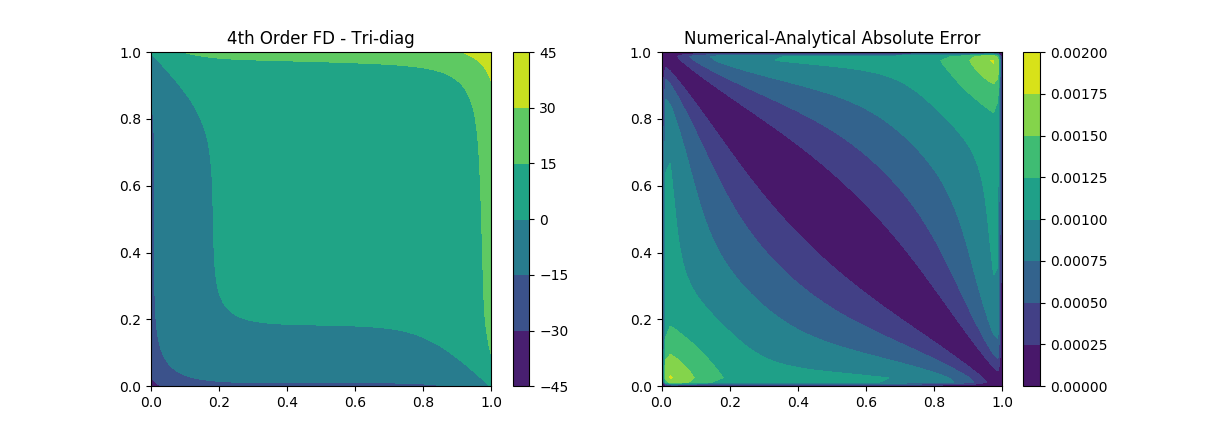
\includegraphics[width=12cm]{./figures/tridiag.png}

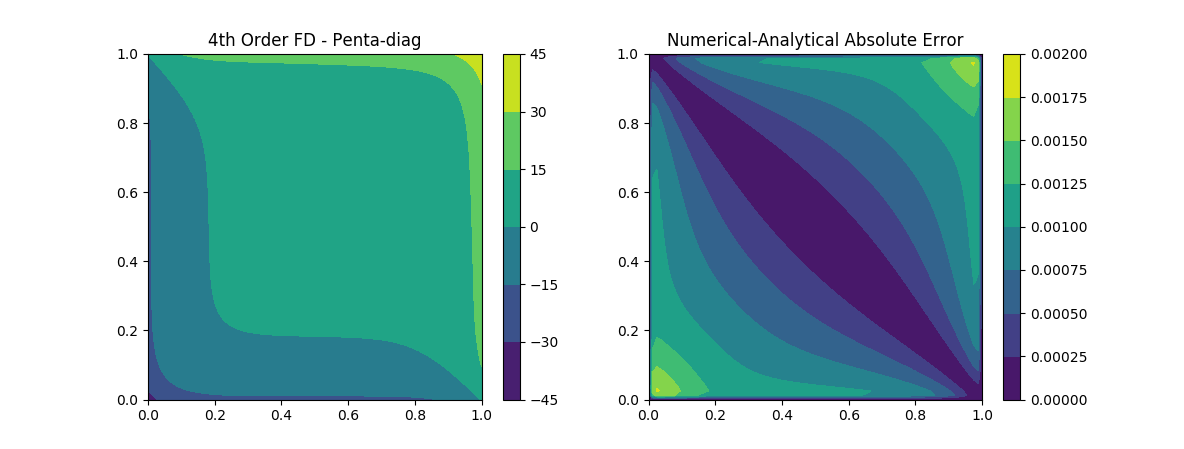
\includegraphics[width=12cm]{./figures/penta.png}

We can see that the maximal error is below 0.002 throughout the domain for both solvers. In fact, due to the convergence criterion being so tight, no perceivable difference can be seen between the contour plots of both solvers.
A satisfying 3d plot is shown, to show the geometrical complexity of the given problem.

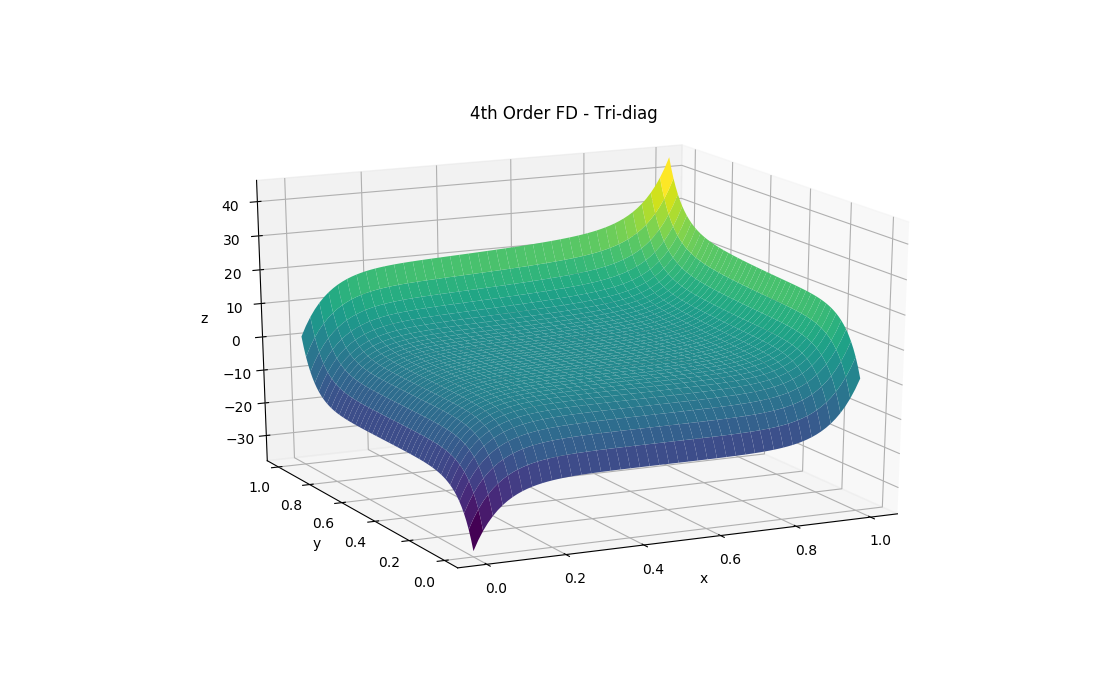
\includegraphics[width=12cm]{./figures/3d.png}

The residual was computed at each iteration and is plotted over the course of the computation.

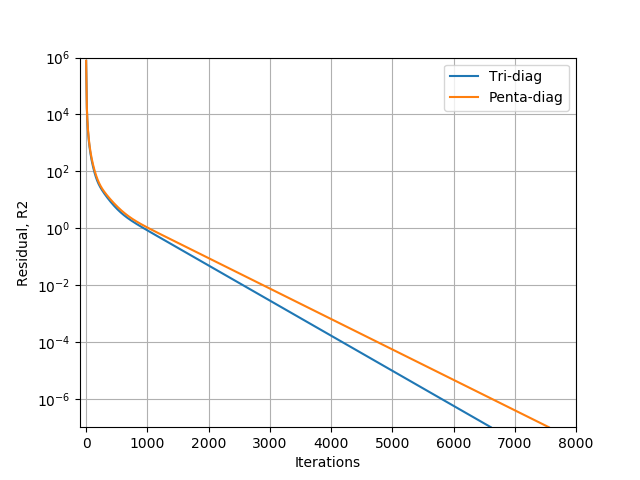
\includegraphics[width=12cm]{./figures/residual.png}

Interestingly we find that the tridiagonal ADI scheme converges faster than pentadiagonal ADI scheme. This affirms that the tridiagonal method is an ideal candidate for solving Poisson equations with high order central differencing schemes.

Lastly we will take a look at running times of the tridiagonal ADI code (see appendix for code) using pure Python, and Numba optimized code.

\begin{center}
\begin{tabular}{lrl}
\hline
Configuration & Runtime [s] & \% of baseline\\
\hline
Pure Python & 288 & 100 \%\\
Numba & 8.5 & 2.9\%\\
\hline
\end{tabular}
\end{center}
We see a speed of over 33X by utilizing Numba, showing the great potential Numba has for numerical computing.
It is important to note that this comparison used the vectorized l2Norm, and not the naive double for loop implementation. It is safe to assume that the performance gap using the non-vectorized approach would be even larger than observed here.

\newpage
\section{Appendix: Python Code}
\label{sec-2}
\begin{minted}[]{python}
import matplotlib.pyplot as plt
import numpy as np
import math
from scipy.linalg import *
from numba import jit, prange
from mpl_toolkits.mplot3d import Axes3D
from matplotlib import cm

@jit
def trirowstepper(phi, S, phi_left, phi_right, phi_bottom, phi_top, dx2, dy2):
    nx, ny = phi.shape
    phin = np.copy(phi)
    d = np.zeros(nx, dtype=float)
    Q = np.zeros(nx,dtype=float)
    c = np.zeros(nx-1,dtype=float)
    a = np.zeros(nx-1,dtype=float)
    for j in range(1, ny-1):
	if j == 1 or j == ny - 2:
	    for i in range(nx):
		if i == 0:
		    d[i] = 1.0
		    c[i] = 0.0
		    Q[i] = phi_left[j]
		elif i == nx-1:
		    d[i] = 1.0
		    a[i-1] = 0.0
		    Q[i] = phi_right[j]
		else:
		    d[i] = -(2/(dx2) + 2/(dy2))
		    c[i] = 1.0/(dx2)
		    a[i-1] = 1.0/(dx2)
		    Q[i] =  S[j,i] - (1.0/dy2)*(phin[j+1,i]) -(1.0/dy2)*(phi[j-1,i])
	else:
	    for i in range(nx):
		if i == 0:
		    d[i] = 1.0
		    c[i] = 0.0
		    #Q[i] = phi_left[ny -1 - j]
		    Q[i] = phi_left[j]
		elif i == nx-1:
		    d[i] = 1.0
		    a[i-1] = 0.0
		    #Q[i] = phi_right[ny -1 - j]
		    Q[i] = phi_right[j]
		elif ((i == 1) or (i == nx-2)):
		    d[i] = -(2.0/(dx2) + 2.0/(dy2))
		    c[i] = 1.0/(dx2)
		    a[i-1] = 1.0/(dx2)
		    Q[i] =  S[j,i] - (1.0/dy2)*(phin[j+1,i]) -(1.0/dy2)*(phi[j-1,i])
		else:
		    d[i] = -(5.0/(2.0*dx2) + 5.0/(2.0*dy2))
		    c[i] = 4.0/(3.0*dx2)
		    a[i-1] = 4.0/(3.0*dx2)
		    Q[i] =  S[j,i] + (1.0/(12.0*dy2))*(phin[j+2,i] -4*phin[j+1,i] -4*phi[j-1,i] \
			    + phi[j-2,i]) -(1/dy2)*(phin[j+1,i] +phi[j-1,i]) +(1.0/(12*dx2))*(phin[j,i+2] + phi[j,i-2])

	phi[j,:] = tridiag(d, c, a, Q)
    return phi

@jit
def tricolstepper(phi, S, phi_left, phi_right, phi_bottom, phi_top, dx2, dy2):
    nx, ny = phi.shape
    phin = np.copy(phi)
    d = np.zeros(ny, dtype=float)
    Q = np.zeros(ny,dtype=float)
    c = np.zeros(ny-1,dtype=float)
    a = np.zeros(ny-1,dtype=float)
    for i in range(1, nx-1):
	if i == 1 or i == nx - 2:
	    for j in range(ny):
		if j == 0:
		    d[j] = 1.0
		    c[j] = 0.0
		    Q[j] = phi_bottom[i]
		elif j == ny-1:
		    d[j] = 1.0
		    a[j-1] = 0.0
		    Q[j] = phi_top[i]
		else:
		    d[j] = -(2/(dy2) + 2/(dx2))
		    c[j] = 1.0/(dy2)
		    a[j-1] = 1.0/(dy2)
		    Q[j] =  S[j,i] - (1.0/dx2)*(phin[j,i+1]) -(1.0/dx2)*(phi[j,i-1])

	else:
	    for j in range(ny):
		if j == 0:
		    d[j] = 1.0
		    c[j] = 0.0
		    Q[j] = phi_bottom[i]
		elif j == ny-1:
		    d[j] = 1.0
		    a[j-1] = 0.0
		    Q[j] = phi_top[i]
		elif ((j == 1) or (j == ny-2)):
		    d[j] = -(2.0/(dy2) + 2.0/(dx2))
		    c[j] = 1.0/(dy2)
		    a[j-1] = 1.0/(dy2)
		    Q[j] =  S[j,i] - (1.0/dx2)*(phin[j,i+1]) -(1.0/dx2)*(phi[j,i-1])
		else:
		    d[j] = -(5.0/(2.0*dy2) + 5.0/(2.0*dx2))
		    c[j] = 4.0/(3.0*dy2)
		    a[j-1] = 4.0/(3.0*dy2)
		    Q[j] =  S[j,i] + (1.0/(12.0*dx2))*(phin[j,i+2] -4*phin[j,i+1] -4*phi[j,i-1] \
			    + phi[j,i-2]) -(1/dx2)*(phin[j,i+1] +phi[j,i-1]) +(1.0/(12*dy2))*(phin[j+2,i] + phin[j-2,i])

	phi[:,i] = tridiag(d, c, a, Q)
    return phi


@jit
def pentrowstepper(phi, S, phi_left, phi_right, phi_bottom, phi_top, dx2, dy2):
    nx, ny = phi.shape
    phin = np.copy(phi)
    d = np.zeros(nx, dtype=float)
    Q = np.zeros(nx,dtype=float)
    c = np.zeros(nx-1,dtype=float)
    a = np.zeros(nx-1,dtype=float)
    f = np.zeros(nx-2,dtype=float)
    e = np.zeros(nx-2,dtype=float)


    for j in range(1, ny-1):
	if j == 1 or j == ny - 2:
	    for i in range(nx):
		if i == 0:
		    d[i] = 1.0
		    c[i] = 0.0
		    f[i] = 0.0
		    Q[i] = phi_left[j]
		elif i == 1:
		    d[i] = -(2/(dx2) + 2/(dy2))
		    c[i] = 1.0/(dx2)
		    a[i-1] = 1.0/(dx2)
		    f[i] = 0.0
		    Q[i] =  S[j,i] - (1.0/dy2)*(phin[j+1,i]) -(1.0/dy2)*(phi[j-1,i])

		elif i == nx-1:
		    d[i] = 1.0
		    a[i-1] = 0.0
		    e[i-2] = 0
		    Q[i] = phi_right[j]

		elif i == nx-2:
		    d[i] = -(2/(dx2) + 2/(dy2))
		    c[i] = 1.0/(dx2)
		    a[i-1] = 1.0/(dx2)
		    e[i-2] = 0
		    Q[i] =  S[j,i] - (1.0/dy2)*(phin[j+1,i]) -(1.0/dy2)*(phi[j-1,i])

		else:
		    d[i] = -(2/(dx2) + 2/(dy2))
		    c[i] = 1.0/(dx2)
		    a[i-1] = 1.0/(dx2)
		    e[i-2] = 0
		    f[i] = 0
		    Q[i] =  S[j,i] - (1.0/dy2)*(phin[j+1,i]) -(1.0/dy2)*(phi[j-1,i])
	    phi[j,:] = tridiag(d, c, a, Q)
	else:
	    for i in range(nx):
		if i == 0:
		    d[i] = 1.0
		    c[i] = 0.0
		    f[i] = 0.0
		    Q[i] = phi_left[j]
		elif i == 1:
		    d[i] = -(2/(dx2) + 2/(dy2))
		    c[i] = 1.0/(dx2)
		    a[i-1] = 1.0/(dx2)
		    f[i] = 0
		    Q[i] =  S[j,i] - (1.0/dy2)*(phin[j+1,i]) -(1.0/dy2)*(phi[j-1,i])

		elif i == nx-1 :
		    d[i] = 1.0
		    a[i-1] = 0.0
		    e[i-2] = 0
		    Q[i] = phi_right[j]
		elif i == nx-2:
		    d[i] = -(2/(dx2) + 2/(dy2))
		    c[i] = 1.0/(dx2)
		    a[i-1] = 1.0/(dx2)
		    e[i-2] = 0.0
		    Q[i] =  S[j,i] - (1.0/dy2)*(phin[j+1,i]) -(1.0/dy2)*(phi[j-1,i])

		else:
		    d[i] = -(5.0/(2.0*dx2) + 5.0/(2.0*dy2))
		    c[i] = 4.0/(3.0*dx2)
		    a[i-1] = 4.0/(3.0*dx2)
		    f[i] = -(1.0/(12.0*dx2))
		    e[i-2] = -(1.0/(12.0*dx2))
		    Q[i] =  S[j,i] + (1.0/(12.0*dy2))*(phin[j+2,i] -4*phin[j+1,i] -4*phi[j-1,i] \
			    +phi[j-2,i]) -(1/dy2)*(phin[j+1,i] +phi[j-1,i])
	    phi[j,:] = pentadiag(d, f, c, a, e, Q)
    return phi

@jit
def pentcolstepper(phi, S, phi_left, phi_right, phi_bottom, phi_top, dx2, dy2):
    nx, ny = phi.shape
    phin = np.copy(phi)
    d = np.zeros(ny, dtype=float)
    Q = np.zeros(ny,dtype=float)
    c = np.zeros(ny-1,dtype=float)
    a = np.zeros(ny-1,dtype=float)
    f = np.zeros(ny-2,dtype=float)
    e = np.zeros(ny-2,dtype=float)

    for i in range(1, nx-1):
	if i == 1 or i == nx - 2:
	    for j in range(ny):
		if j == 0:
		    d[j] = 1.0
		    c[j] = 0.0
		    f[j] = 0.0
		    Q[j] = phi_bottom[i]
		elif j == 1:
		    d[j] = -(2/(dx2) + 2/(dy2))
		    c[j] = 1.0/(dy2)
		    a[j-1] = 1.0/(dy2)
		    f[j] = 0.0
		    Q[j] =  S[j,i] - (1.0/dx2)*(phin[j,i+1]) -(1.0/dx2)*(phi[j,i-1])

		elif j == ny-1:
		    d[j] = 1.0
		    a[j-1] = 0.0
		    e[j-2] = 0
		    Q[j] = phi_top[i]

		elif j == ny-2:
		    d[j] = -(2/(dx2) + 2/(dy2))
		    c[j] = 1.0/(dy2)
		    a[j-1] = 1.0/(dy2)
		    e[j-2] = 0
		    Q[j] =  S[j,i] - (1.0/dx2)*(phin[j,i+1]) -(1.0/dx2)*(phi[j,i-1])

		else:
		    d[j] = -(2/(dx2) + 2/(dy2))
		    c[j] = 1.0/(dy2)
		    a[j-1] = 1.0/(dy2)
		    e[j-2] = 0
		    f[j] = 0
		    Q[j] =  S[j,i] - (1.0/dx2)*(phin[j,i+1]) -(1.0/dx2)*(phi[j,i-1])
	    phi[:,i] = tridiag(d, c, a, Q)
	else:
	    for j in range(ny):
		if j == 0:
		    d[j] = 1.0
		    c[j] = 0.0
		    f[j] = 0.0
		    Q[j] = phi_bottom[i]
		elif j == 1:
		    d[j] = -(2/(dx2) + 2/(dy2))
		    c[j] = 1.0/(dy2)
		    a[j-1] = 1.0/(dy2)
		    f[j] = 0
		    Q[j] =  S[j,i] - (1.0/dx2)*(phin[j,i+1]) -(1.0/dx2)*(phi[j,i-1])

		elif j == ny-1:
		    d[j] = 1.0
		    a[j-1] = 0.0
		    e[j-2] = 0
		    Q[j] = phi_top[i]
		elif j == ny-2:
		    d[j] = -(2/(dx2) + 2/(dy2))
		    c[j] = 1.0/(dy2)
		    a[j-1] = 1.0/(dy2)
		    e[j-2] = 0.0
		    Q[j] =  S[j,i] - (1.0/dx2)*(phin[j,i+1]) -(1.0/dx2)*(phi[j,i-1])

		else:
		    d[j] = -(5.0/(2.0*dx2) + 5.0/(2.0*dy2))
		    c[j] = 4.0/(3.0*dy2)
		    a[j-1] = 4.0/(3.0*dy2)
		    f[j] = -(1.0/(12.0*dy2))
		    e[j-2] = -(1.0/(12.0*dy2))
		    Q[j] =  S[j,i] + (1.0/(12.0*dx2))*(phin[j,i+2] -4*phin[j,i+1] \
			    -4*phi[j,i-1] +phi[j,i-2]) -(1/dx2)*(phin[j,i+1] +phi[j,i-1])

	    phi[:,i] = pentadiag(d, f, c, a, e, Q)
    return phi

@jit
def tridiag(d, c, a, Q):
    N = len(Q)
    ans = np.zeros(N)
    d = np.copy(d)
    c = np.copy(c)
    a = np.copy(a)
    Q = np.copy(Q)

    for i in range(1,N):
	const = a[i-1]/d[i-1]
	d[i] = d[i] - const*c[i-1]
	Q[i] = Q[i] - const*Q[i-1]
    ans[N-1] = Q[N-1]/d[N-1]
    for i in range(N-2, -1, -1):
	ans[i] = (Q[i] -c[i]*ans[i+1])/d[i]
    return ans

@jit
def pentadiag(d, f, c, a, e, Q):
    N = len(Q)
    ans = np.zeros(N)
    d = np.copy(d)
    f = np.copy(f)
    c = np.copy(c)
    a = np.copy(a)
    e = np.copy(e)
    Q = np.copy(Q)

    for i in range(1, N-1):
	const1 = a[i-1]/d[i-1]
	d[i] = d[i] -const1*c[i-1]
	c[i] = c[i] -const1*f[i-1]
	Q[i] = Q[i] -const1*Q[i-1]
	const2 = e[i-1]/d[i-1]
	a[i] = a[i] -const2*c[i-1]
	d[i+1] = d[i+1] -const2*f[i-1]
	Q[i+1] = Q[i+1] - const2*Q[i-1]
    const3 = a[N-2]/d[N-2]
    d[N-1] = d[N-1] -const3*c[N-2]
    ans[N-1] = (Q[N-1] -const3*Q[N-2])/d[N-1]
    ans[N-2] = (Q[N-2] -c[N-2]*Q[N-1])/d[N-2]
    for i in range(N-3, -1, -1):
	ans[i] = (Q[i] -c[i]*ans[i+1] -f[i]*ans[i+2])/d[i]
    return ans
    # c = np.concatenate([[0],c])
    # f = np.concatenate([[0,0],f])
    # a = np.concatenate([a,[0]])
    # e = np.concatenate([e,[0,0]])
    # ab = np.matrix([f,c, d, a, e])                  # simplified matrix
    # ans = solve_banded((2, 2), ab, Q)
    # return ans
@jit
def l2norm(phi, dx2, dy2):
   ny, nx = phi.shape
   Rk = phi[2:-2,2:-2]*(-(5.0/(2.0*dx2) + 5.0/(2.0*dy2))) + phi[2:-2,3:-1]*(4.0/(3.0*dx2)) \
	+ phi[2:-2,1:-3]*(4.0/(3.0*dx2)) + phi[3:-1,2:-2]*(4.0/(3.0*dy2)) \
	+ phi[1:-3,2:-2]*(4.0/(3.0*dy2)) + phi[2:-2,4:]*(-1.0/(12*dx2)) + \
	phi[2:-2,:-4]*(-1.0/(12*dx2)) + phi[4:,2:-2]*(-1.0/(12*dy2)) \
	+ phi[:-4,2:-2]*(-1.0/(12*dy2))
   Rksquared = np.multiply(Rk,Rk)
   return math.sqrt(Rksquared.sum())


if __name__ == "__main__":
    nx = 81
    ny = 81
    dx = 1/(nx-1)
    dx2 = dx**2
    dy = 1/(ny-1)
    dy2 = dy**2

    epsilon = 10e-8
    maxiters = 8000

    x = np.linspace(0, 1, nx)
    y = np.linspace(0, 1, ny)
    xx, yy = np.meshgrid(x, y, sparse=True)

    # Expressions
    phi_analytical = ((xx -0.5)**2)*np.sinh(10*(xx-0.5)) \
		     + ((yy-0.5)**2)*np.sinh(10*(yy-0.5)) + np.exp(2*xx*yy)
    S = 2*np.sinh(10*(xx-0.5)) + 40*(xx-0.5)*np.cosh(10*(xx-0.5)) \
	+ 100*((xx-0.5)**2)*np.sinh(10*(xx-0.5)) + 2*np.sinh(10*(yy-0.5)) \
	+ 40*(yy-0.5)*np.cosh(10*(yy-0.5)) \
	+ 100*((yy-0.5)**2)*np.sinh(10*(yy-0.5)) \
	+ 4*(xx**2 + yy**2)*np.exp(2*xx*yy)
    phi_left = 0.25*np.sinh(-5) + ((y-0.5)**2)*np.sinh(10*(y-0.5)) + 1
    phi_right = 0.25*np.sinh(5) + ((y-0.5)**2)*np.sinh(10*(y-0.5)) + np.exp(2*y)
    phi_bottom = 0.25*np.sinh(-5) + ((x-0.5)**2)*np.sinh(10*(x-0.5)) + 1
    phi_top = 0.25*np.sinh(5) + ((x-0.5)**2)*np.sinh(10*(x-0.5)) + np.exp(2*x)


    phi = np.zeros((ny,nx), dtype=float)
    phi[0,:] = phi_bottom
    phi[ny-1,:] = phi_top
    phi[:, 0] = phi_left
    phi[:, nx-1] = phi_right
    phistart = phi.copy()


    # Tridiag solve
    phiold = phi.copy()
    l2norm_phi = np.zeros(maxiters)
    for iteration in range(maxiters):
	phi = trirowstepper(phi, S, phi_left, phi_right, phi_bottom, phi_top, dx2, dy2)
	phi = tricolstepper(phi, S, phi_left, phi_right, phi_bottom, phi_top, dx2, dy2)
	l2norm_phi[iteration] = l2norm(phi-phiold, dx2, dy2)
	if l2norm_phi[iteration] < epsilon:
	    break
	phiold = phi.copy()
    phi_tri = phi.copy()
    l2norm_tri = l2norm_phi.copy()

    # Pentadiag solve
    phi = np.copy(phistart)
    phiold = np.copy(phistart)
    l2norm_phi = np.zeros(maxiters)
    for iteration in range(maxiters):
	phi = pentrowstepper(phi, S, phi_left, phi_right, phi_bottom, phi_top, dx2, dy2)
	phi = pentcolstepper(phi, S, phi_left, phi_right, phi_bottom, phi_top, dx2, dy2)
	l2norm_phi[iteration] = l2norm(phi-phiold, dx2, dy2)
	if l2norm_phi[iteration] < epsilon:
	    break
	phiold = phi.copy()
    phi_penta = phi.copy()
    l2norm_penta = l2norm_phi.copy()

    plt.figure(1)
    plt.subplot(121)
    plt.contourf(x,y,phi_tri)
    plt.colorbar()
    plt.title('4th Order FD - Tri-diag')
    plt.subplot(122)
    plt.contourf(x,y,np.abs(phi_analytical-phi_tri))
    plt.colorbar()
    plt.title('Numerical-Analytical Absolute Error')

    plt.figure(2)
    plt.subplot(121)
    plt.contourf(x,y,phi_penta)
    plt.colorbar()
    plt.title('4th Order FD - Penta-diag')
    plt.subplot(122)
    plt.contourf(x,y,np.abs(phi_analytical-phi_penta))
    plt.colorbar()
    plt.title('Numerical-Analytical Absolute Error')

    plt.figure(3)
    plt.semilogy(np.arange(len(l2norm_tri))*2, l2norm_tri, label="Tri-diag")
    plt.semilogy(np.arange(len(l2norm_penta))*2, l2norm_penta, label="Penta-diag")
    plt.xlim((-100,8000))
    plt.ylim((0,10**6))
    plt.xlabel("Iterations")
    plt.ylabel("Residual, R2")
    plt.legend()
    plt.grid(True)
    plt.show()

    fig = plt.figure(figsize=(11, 7), dpi=100)
    ax = fig.gca(projection='3d')
    ax.plot_surface(xx, yy, phi_tri, cmap=cm.viridis, rstride=2, cstride=2)
    ax.set_xlabel('x')
    ax.set_ylabel('y')
    ax.set_zlabel('z')
    plt.title('4th Order FD - Tri-diag')
    plt.show()
\end{minted}
% Emacs 25.3.1 (Org mode 8.2.10)
\end{document}